%%%%%%%%%%%%
%
% $Autor: Adhiraj $
% $Datum: 2025-01-15 08:03:15Z $
% $Pfad: Results $
% $Version: 4250 $
% !TeX spellcheck = en_GB/de_DE
% !TeX encoding = utf8
% !TeX root = Results 
% !TeX TXS-program:bibliography = txs:///biber
%
%%%%%%%%%%%%
\chapter{Evaluation and Verification}

Once we get the model ready, it is important to test the model with a different dataset. This helps us confirm our model will work fine with gestures from other persons as well. To test the model we need to now call the Keras's \textcolor{red}{model.evaluate()} function.\cite{Warden:2020}

We can also use a confusion matrix to check the performance of the model. An example of a confusion matrix according to the \cite{Warden:2020} is shown below which is calculated by \textcolor{red}{ tf.math.confusion$\_$matrix()} function:

\[
\text{{tf.Tensor}} \left(
\begin{bmatrix}
	75 & 3 & 0 & 4 \\
	0 & 69 & 0 & 15 \\
	0 & 0 & 85 & 3 \\
	0 & 0 & 1 & 129 \\
\end{bmatrix},
\text{{shape}}=(4, 4),
\text{{dtype}}=\text{{int32}}
\right)
\]

The confusion matrix function assesses the accuracy of the predicted class for each input in the test dataset by comparing it to the actual class. It reveals the model's limitations, pinpointing areas that need improvement. By leveraging this feedback, we can adjust the dataset and retrain the model, leading to continuous performance enhancement as the model learns from its mistakes \cite{Warden:2020}.

\chapter{Results}
\label{Results}
After considerable effort in building a comprehensive dataset and training the model, the Magic Wand project, powered by the Arduino Nano BLE 33 sensor, demonstrated promising results during implementation. The gesture recognition system accurately identified and responded to predefined gestures, specifically W (Wing), O (Ring), and L (Slope). This successful integration of TinyML with the Arduino platform highlights the potential for real-time, edge-based gesture recognition in interactive applications, marking a significant step forward in utilizing machine learning for intuitive control systems.

\begin{itemize}
	
	\item \textbf{Gesture Recognition:}
	
	The system demonstrated a strong capability in recognizing predefined gestures: W (Wing) \ref{fig: Result for Wing Gesture}, O (Ring) \ref{fig: Result for Ring Gesture}, and L (Slope) \ref{fig: Result for Slope Gesture}. By adding an "Unknown" category for unrecognized movements, the project gained greater flexibility and adaptability to different gestures.
	
	\item \textbf{LED Feedback:}
	
	Real-time visual feedback through LED lights in red \ref{fig: Result for Wing Gesture with Red Light}, green \ref{fig: Result for Ring Gesture with Green Light}, blue \ref{fig: Result for Unknown Gesture}, and white \ref{fig: Result for Unknown Gesture with White Light} reinforced the accuracy of gesture recognition. This feedback not only improved the user experience but also acted as a clear indicator of system performance.
	
	\item \textbf{Challenges Overcome:}
	
	The development journey wasn't without its hurdles. Initially, the model struggled with precise gesture recognition. However, these issues were addressed by consistently refining data collection methods, improving model training processes, and optimizing the code for better performance.
	
	\item \textbf{Iterative Refinement:}
	
	The project’s success can largely be attributed to its iterative approach. Through repeated adjustments to the dataset, careful model tuning, and code improvements, the project achieved significant progress in gesture recognition accuracy.
	
	\item \textbf{Accomplishments:}
	
	Despite facing early challenges, the Magic Wand project is now a successful example of integrating hardware with machine learning to enable gesture-based interactions. The project demonstrates the potential for real-time, accurate gesture recognition using TinyML.
	
	\item \textbf{Visual Representation:}
	
	Enclosed are images that capture moments when recognized gestures are triggered, providing a visual insight into the successful implementation of the project.
	
\end{itemize}

\begin{figure}[H]
	\centering
	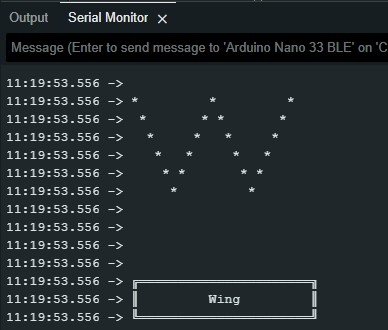
\includegraphics[height = 120 mm, width=100mm]{Images/Results/Wing}
	\caption{Gesture Output for WING \textbf{W} on Output Terminal } 
	\label{fig: Result for Wing Gesture}
\end{figure}

\begin{figure}[H]
	\centering
	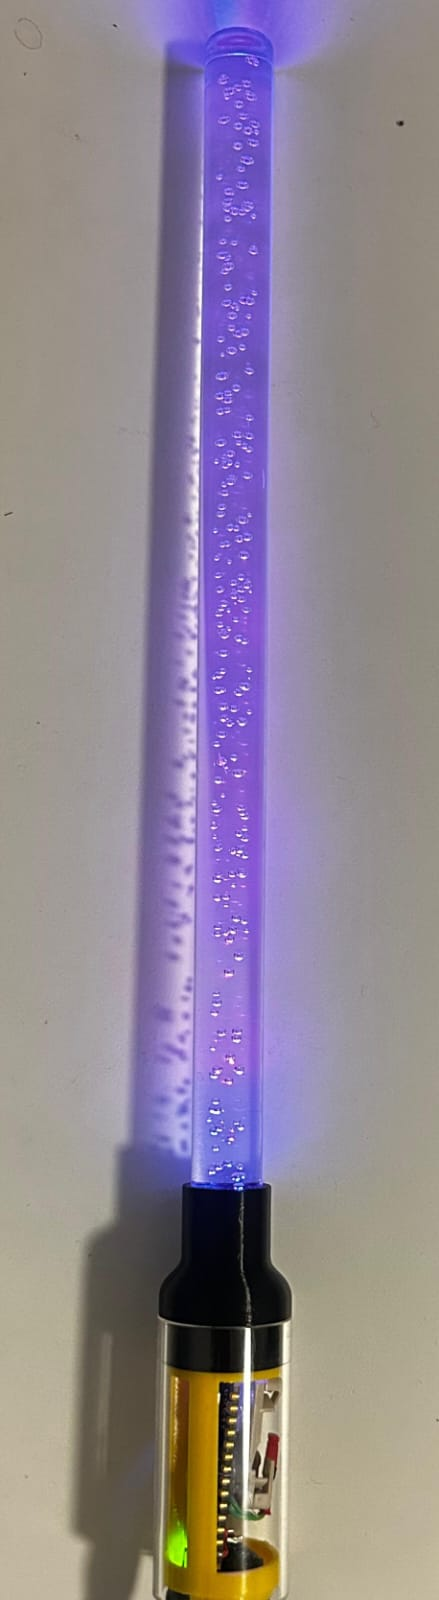
\includegraphics[height = 150 mm, width=50mm]{Images/Results/Red}
	\caption{RED Colour Output for WING \textbf{W} on Magic Wand} 
	\label{fig: Wand Colour for Wing Gesture}
\end{figure}

\begin{figure}[H]
	\centering
	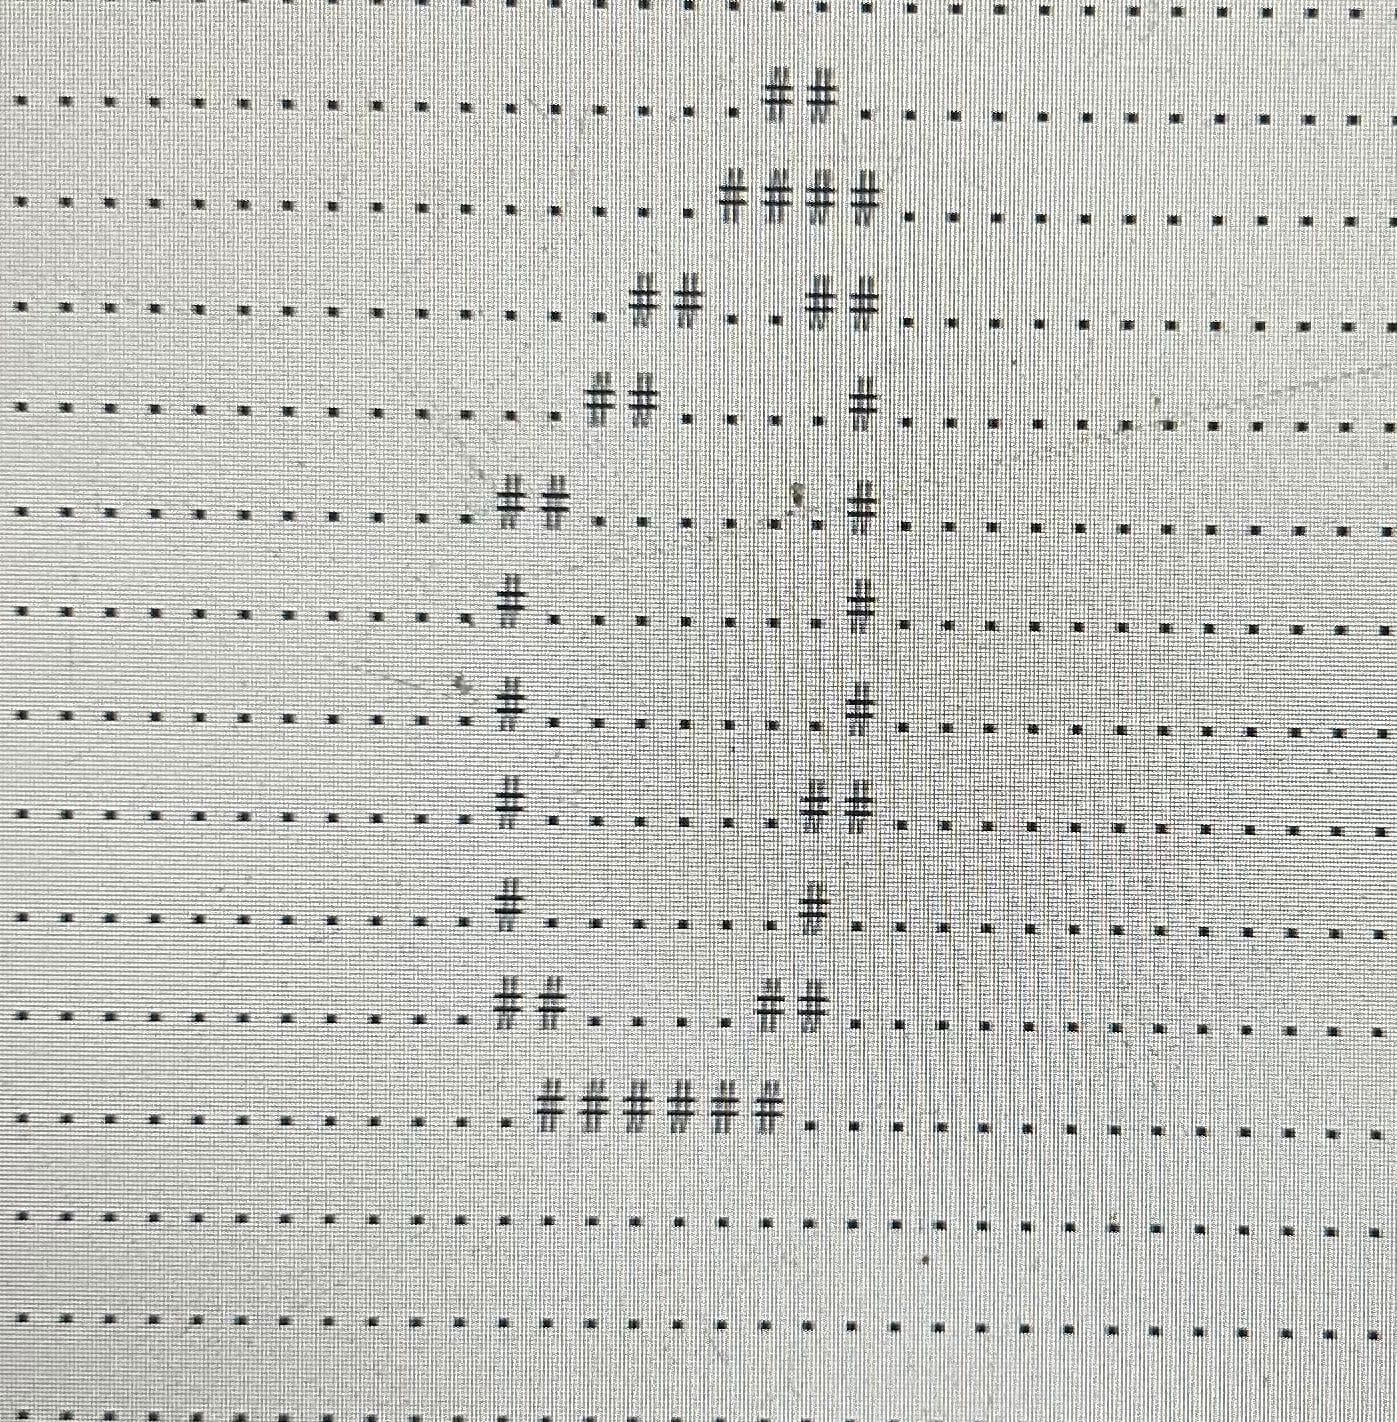
\includegraphics[height = 120 mm, width=100mm]{Images/Results/Ring}
	\caption{Gesture Output for RING \textbf{O} on Output Terminal } 
	\label{fig: Result for Ring Gesture}
\end{figure}

\begin{figure}[H]
	\centering
	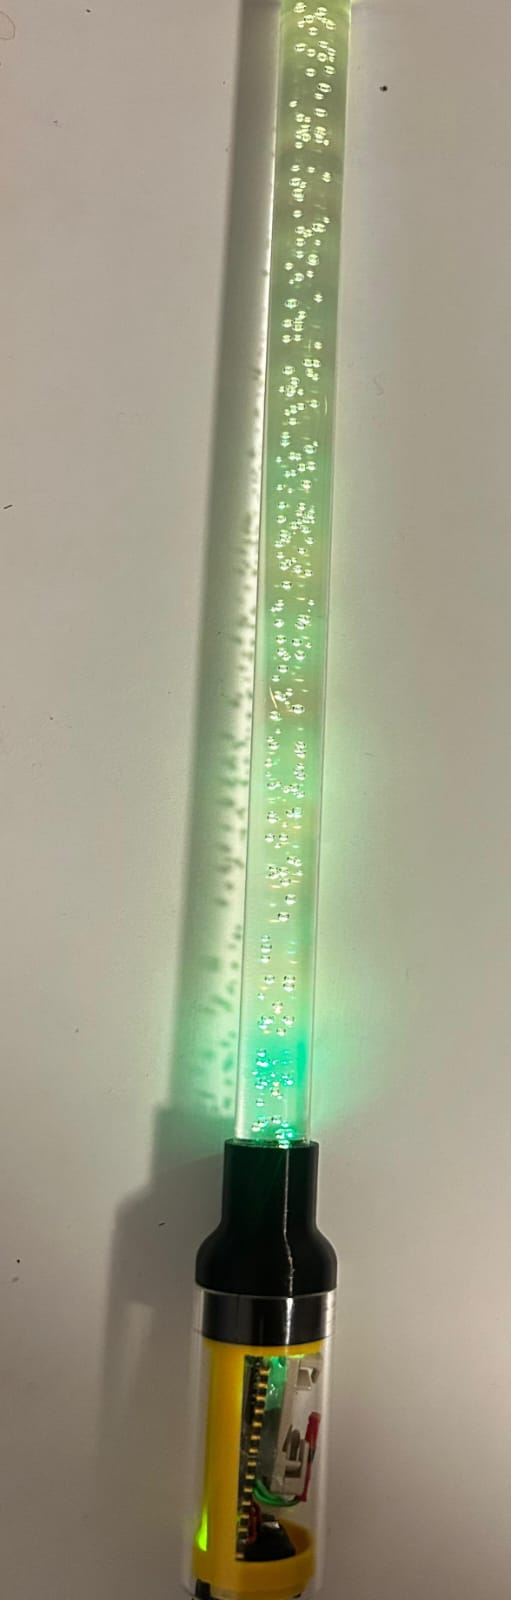
\includegraphics[height = 170 mm, width=50mm]{Images/Results/Green}
	\caption{GREEN Colour Output for RING \textbf{O} on Magic Wand } 
	\label{fig: Wand Colour for Ring Gesture}
\end{figure}

\begin{figure}[H]
	\centering
	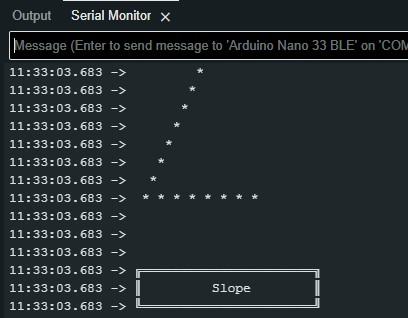
\includegraphics[height = 160 mm, width=90mm]{Images/Results/Slope}
	\caption{Gesture Output for  SLOPE \textbf{L} on Output Terminal } 
	\label{fig: Result for Slope Gesture}
\end{figure}

\begin{figure}[H]
	\centering
	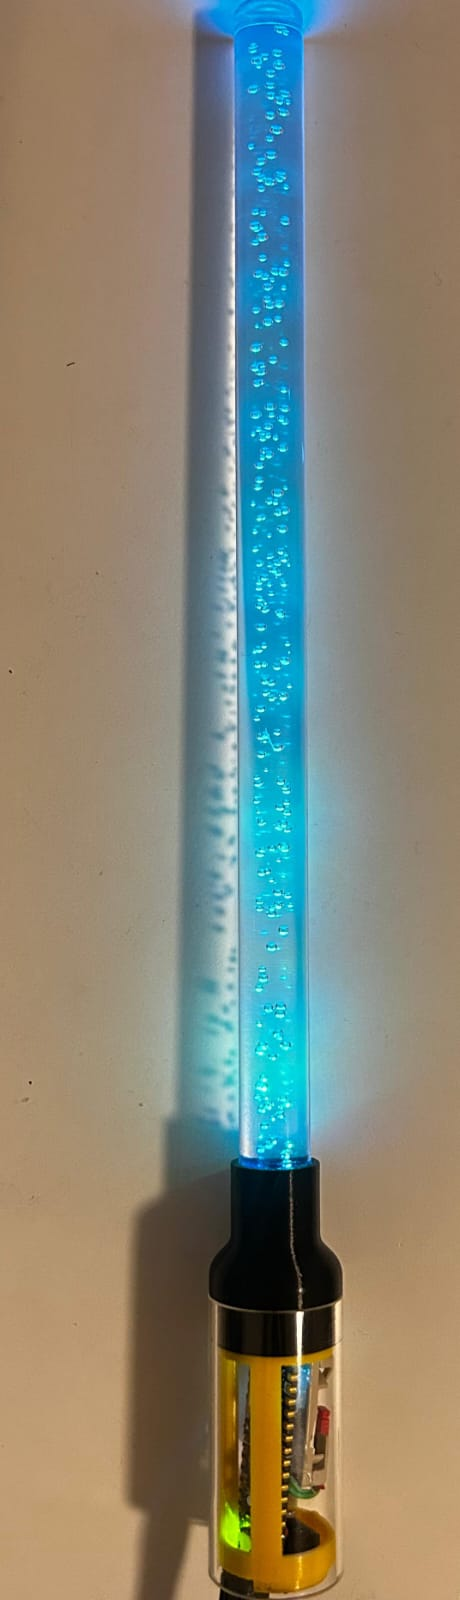
\includegraphics[height = 170 mm, width=50mm]{Images/Results/Blue}
	\caption{BLUE Colour Output for  SLOPE \textbf{L} on Magic Wand } 
	\label{fig: Wand Colour for Slope Gesture}
\end{figure}

\chapter{Conclusion}
\label{Conclusion}

In conclusion, the integration of Tiny Machine Learning (TinyML) with the Arduino Nano 33 BLE Sense has paved the way for the development of a unique and interactive "Magic Wand." This project signifies the synergy between machine learning advancements and the versatile capabilities of edge devices in the realm of the Internet of Things (IoT). The ability to process data locally, demonstrated through gesture recognition on the Arduino board, showcases the potential of edge computing in responding instantly to user inputs.

The implementation involves TensorFlow Lite, which contributes to the success of gesture recognition by utilizing a Neural Network model. The incorporation of a heuristic function adds an element of customization, allowing users to define and refine gesture knowledge without extensive programming skills. The visual output of recognized gestures and the LED response underscore the real-time interaction achieved through this integration.

Despite the challenges encountered during the planning process, such as managing the data model size within the Arduino Nano 33 BLE Sense's memory limitations and training for accuracy, the project's success demonstrates the feasibility of deploying machine learning applications on resource-constrained platforms.

\begin{enumerate}
\item \textbf{Accuracy Enhancement:} 
Focus on refining the algorithms or machine learning models to improve the accuracy and reliability of gesture recognition, minimizing both false positives and negatives. Furthermore, the script has been updated to integrate an LED output as an additional result of the gesture recognition, providing an alternate output view alongside the Arduino IDE serial output monitor.

\item \textbf{Enrichment of the testing procedures:} 
The testing process now specifies the exact aspects being tested (e.g., accuracy of motion detection and responsiveness of LEDs). We have documented the hardware setup, including all necessary connections and the test environment. Clear, step-by-step instructions for conducting the tests are provided, including relevant code snippets or commands. Expected outcomes are clarified, with specific values or behaviors that indicate successful testing.

\item \textbf{Optimized the code listing:} 
The complete code used for testing has been significantly improved, with key sections explained in detail beneath the code. This enhances readability and provides comprehensive guidance for understanding the experiments, ensuring that the process is accessible and well-documented for future reference.

\item \textbf{Enhancement of the test results:} 
The results from the hardware are documented thoroughly, including images of the serial monitor outputs and visual indicators used during testing to demonstrate that the code is functioning as expected. The experiments are interpreted, confirming the reliability of the tested components and providing insights into the overall system performance.

\item \textbf{Software Description Enrichment:} 
A sensor calibration code has been added to the software suite. Calibration is critical for ensuring accurate sensor readings by correcting any inherent hardware deviations or inaccuracies. This step not only enhances the precision of our data collection but also establishes a higher standard for data integrity and reliability, which is essential for subsequent analyses and applications.

\end{enumerate}

\section{Additions}

\begin{enumerate}
	\item \textbf{User Feedback:} 
	Enhance the user interaction by incorporating auditory or haptic feedback during the gesture recognition process. This improvement will provide users with a more immersive and responsive experience, making the system more intuitive to use.
	
	\item \textbf{Expansion of Gesture Library:} 
	Extend the current gesture library to include more complex and diverse motions, enabling the recognition of a wider range of gestures. This expansion will allow users to perform more nuanced actions, enhancing the versatility and functionality of the system.
	
	\item \textbf{Energy Efficiency Improvements:} 
	Introduce energy-saving features to optimize the device's battery life, which is especially critical for portable or wearable applications. This includes techniques such as power-down modes and efficient processing to reduce overall power consumption.
	
	\item \textbf{Environmental Adaptability:} 
	Increase the system’s robustness to varying environmental conditions, such as different lighting, backgrounds, and noise levels, to maintain consistent gesture recognition performance. This will make the device more reliable in real-world settings where conditions often change.
	
	\item \textbf{Community Engagement:} 
	Create an online platform where users can share custom gestures and application ideas. This will foster a collaborative community around the project, enabling others to contribute, improve, and personalize their gesture-based experiences.
\end{enumerate}

\section{To-Do List}

For the next phase of the Magic Wand project using the Arduino Nano 33 BLE Sense, we plan to tackle the following tasks:

\begin{enumerate}
	
	\item \textbf{Design of Enclosure:}
	
	\begin{itemize}
		\item Design and develop a custom enclosure to house the Arduino Nano 33 BLE Sense and the associated components.
		\item Ensure the enclosure is ergonomic and facilitates easy interaction with the wand while providing sufficient protection for the internal components.
	\end{itemize}
	
	\item \textbf{Power Supply Management:}
	
	\begin{itemize}
		\item Calculate the power requirements of the entire system and select an appropriate power supply that meets those needs.
		\item Evaluate the possibility of making the project battery-powered and implement an efficient power management system to prolong battery life during use.
	\end{itemize}
	
	\item \textbf{Stability of Connections:}
	
	\begin{itemize}
		\item Test the connection stability between the Arduino Nano 33 BLE Sense and any peripheral components to ensure reliable communication throughout the system.
		\item Resolve any issues related to unstable or loose connections, ensuring smooth and uninterrupted functionality.
	\end{itemize}
	
	\item \textbf{Physical Attachment and Comfort:}
	
	\begin{itemize}
		\item Securely attach the Arduino Nano 33 BLE Sense to the wand, considering factors such as weight distribution, balance, and ease of use.
		\item Test the attachment to ensure that it can withstand typical handling and use without any risk of detachment or damage.
	\end{itemize}
	
	\item \textbf{Testing and Calibration:}
	
	\begin{itemize}
		\item Calibrate all sensors and components to ensure that the gesture recognition system is accurate and reliable.
		\item Conduct comprehensive testing of the entire hardware setup to identify and address any potential issues before final deployment.
	\end{itemize}
	
	\item \textbf{Comprehensive Documentation:}
	
	\begin{itemize}
		\item Develop thorough documentation for the hardware setup, including assembly instructions, troubleshooting guides, and maintenance tips to ensure ease of use.
		\item Include clear instructions on how to replace batteries (if applicable) and perform other necessary maintenance tasks to keep the system running smoothly.
	\end{itemize}
	
	\item \textbf{Safety and Compliance:}
	
	\begin{itemize}
		\item Ensure that the project complies with relevant safety standards and industry regulations.
		\item Introduce safety features, such as emergency shutdown procedures or safeguards, if applicable, to ensure user safety during operation.
	\end{itemize}
	
	\item \textbf{Packaging and Presentation:}
	
	\begin{itemize}
		\item Design attractive and protective packaging for the Magic Wand that enhances its presentation and ensures it remains secure during shipping.
		\item Consider branding and labeling options to create a professional and polished look for the final product.
	\end{itemize}
	
\end{enumerate}

\section{Unanswered Points}

\begin{enumerate}
	\item \textbf{Device Durability:} 
	There are still questions surrounding the long-term durability and reliability of the device under continuous use. The impact of regular usage on its components, especially over time, needs further investigation.
	
	\item \textbf{User Customization:} 
	The degree of customization available to users for personal preferences, such as customizing gestures and feedback mechanisms, is yet to be fully defined. For instance, our data model has been optimized for users who can perform gestures steadily and at a regular speed, but the system’s performance may be impacted by users who have more erratic hand movements. This needs further analysis to address the recognition accuracy for such cases.
	
	\item \textbf{Data Privacy and Security:} 
	There is a need for clarification on how user data, particularly gesture inputs, are handled and protected against unauthorized access. This includes defining the measures in place to secure sensitive information.
	
	\item \textbf{Cross-Platform Compatibility:} 
	Uncertainties remain regarding the system’s compatibility with various operating systems and devices. Further testing is required to ensure smooth integration without encountering compatibility issues across multiple platforms.
	
	\item \textbf{Real-World Usability:} 
	We need to explore the system’s effectiveness in a variety of real-world scenarios and environments. Its performance in different lighting conditions, user settings, and diverse interaction styles has yet to be fully tested.
	
	\item \textbf{Expansion of Gesture Recognition:} 
	While additional gestures are being considered for inclusion in the data model to enhance recognition capabilities, the potential challenges around the model's capacity to handle diverse and complex gestures need further investigation. This includes examining the limits of gesture resistance and whether the model can effectively handle additional types.
\end{enumerate}

\section{Next Steps}

In the next phase, we aim to address the unanswered points and expand the scope of the project. Key actions include gathering diverse user data and testing new, more complex gestures for broader use cases.

\begin{enumerate}
	\item \textbf{Field Testing:} 
	Conduct extensive field testing to assess the system’s performance in real-world environments, gathering valuable user feedback to guide further improvements.
	
	\item \textbf{Model Refinement:} 
	Refine the machine learning models using real-world data collected from testing, aiming to enhance the accuracy and robustness of gesture recognition.
	
	\item \textbf{Expand Application Ecosystem:} 
	Develop and integrate new applications that take full advantage of the Magic Wand’s gesture recognition capabilities, exploring a wider array of use cases and possibilities.
	
	\item \textbf{Partnerships and Collaborations:} 
	Seek potential partnerships with technology companies and academic institutions to explore innovative technologies and broaden the project’s impact and reach.
	
	\item \textbf{Sustainability Initiatives:} 
	Implement strategies to ensure the sustainability of the project, such as incorporating energy-efficient design practices and using recyclable or eco-friendly materials.
\end{enumerate}

\section{Future Work}

Although our current model is trained to recognize only three distinct gestures, there is considerable potential for expanding its functionality to recognize a broader range of gestures, based on evolving requirements.

Future developments of the project may include the following:

\begin{enumerate}
	\item \textbf{LED Blinking for Specific Gestures:} 
	Implement a feature where the LED attached to the Magic Wand blinks in response to a specific gesture. For instance, a particular gesture could trigger a distinct blinking pattern (e.g., slow blinking for "Wing" gesture, fast blinking for "Ring" gesture). This visual feedback can enhance the user experience, making the system's response more intuitive and noticeable. The LED blinking can also serve as a form of confirmation, ensuring the user that the gesture was recognized.
	
	\item \textbf{Integration of External AI Software:} 
	We plan to explore the possibility of using advanced AI software platforms to further train the model, thereby improving the accuracy of gesture recognition. Additionally, these platforms could help optimize the size of the data model, making it more efficient while retaining high performance.
	
	\item \textbf{Wireless Communication Using BLE:} 
	Leveraging the Bluetooth Low Energy (BLE) capability of the Arduino Nano 33 BLE Sense, we aim to enable wireless communication between the Magic Wand and a computer. This would enhance the system's flexibility, allowing for remote control or interaction without the need for physical connections.
	
	\item \textbf{Advancements in TinyML:} 
	As TinyML technologies continue to evolve, we anticipate greater advancements that can significantly improve the performance of our system. With future improvements in TinyML hardware, such as larger local memory storage and even smaller physical sizes, the capabilities of the Magic Wand could be further enhanced, enabling more sophisticated operations with minimal power consumption.
\end{enumerate}
